\section{Results}
The performance of our algorithm is demonstrated on \philbs and \rphumanserum.
Please refer to section S\ref{S-sec:algorithm_performance} for all other datasets.
For each comparison, the unregularized case is not smoothed, effectively $\lambda = 0$,
the partially regularized case uses the grid search fitted values of $\mathbf{\tau}$ but
uses a fixed $\lambda = 0.2$, and the fully regularized case uses the grid search fitted
values of both $\mathbf{\tau}$ and $\lambda$.

\subsection{Chromatogram Assignment Performance for \philbs}
    The fitted parameters for the network constructed for \philbs are shown in
    Table~\ref{tab:philbs_parameters}. The assigned chromatograms and their qunatification
    are shown in Figure~\ref{fig:philbs_assignments}. The comparison of assignment performance
    with differing degrees of smoothing is shown n Figure~\ref{fig:philbs_perf}. The ROC AUC
    for the unreularized case is 0.838, for the partially regularized case is 0.987, and for
    the fully regularized case is 0.921.

    \begin{table}[h]
        \begin{threeparttable}
            \caption{Fitted $\lambda$, $\gamma$, and $\mathbf{\tau}$ for
                     \philbs \label{tab:philbs_parameters}}
            \begin{tabular}{l l}
                \toprule    
                Neighborhood Name & $\tau_i$ \\
                \midrule
                high-mannose & 17.615084 \\
                hybrid & 13.599120 \\
                bi-antennary & 0.0 \\
                asialo-bi-antennary & 13.919251 \\
                tri-antennary & 0.0 \\
                asialo-tri-antennary & 12.906467 \\
                tetra-antennary & 0.0 \\
                asialo-tetra-antennary & 14.723146 \\
                penta-antennary & 0.0 \\
                asialo-penta-antennary & 11.226188 \\
                hexa-antennary & 0.0 \\
                asialo-hexa-antennary & 10.696785 \\
                hepta-antennary & 0.0 \\
                asialo-hepta-antennary & 3.071313 \\
                \bottomrule
            \end{tabular}
            \begin{tablenotes}[normal]
                \item Fitted $\lambda = 0.99$ and $\gamma = 11.12$.
            \end{tablenotes}
        \end{threeparttable}
    \end{table}

    \begin{figure}[h]
        \caption{Chromatogram Assignments and Quantification
                 for \philbs\label{fig:philbs_assignments}}
        \centering
        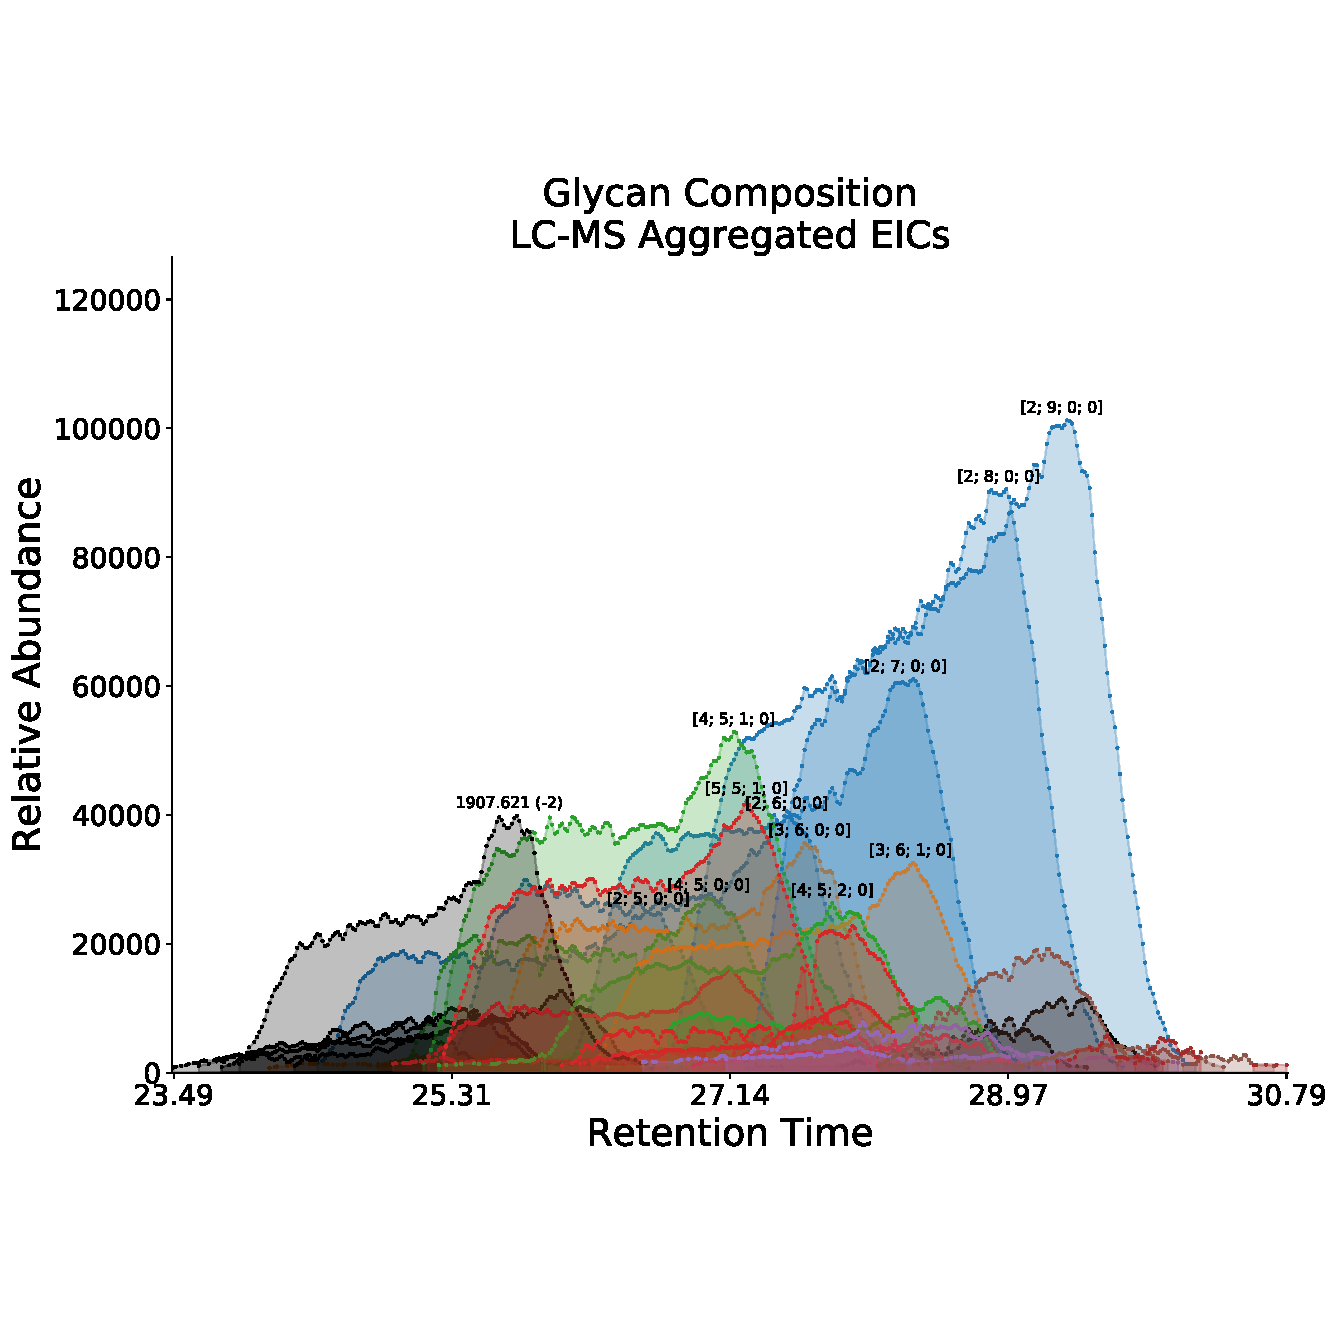
\includegraphics[width=0.45\textwidth,valign=t]{figure/phil_bs_chromatograms.pdf}
        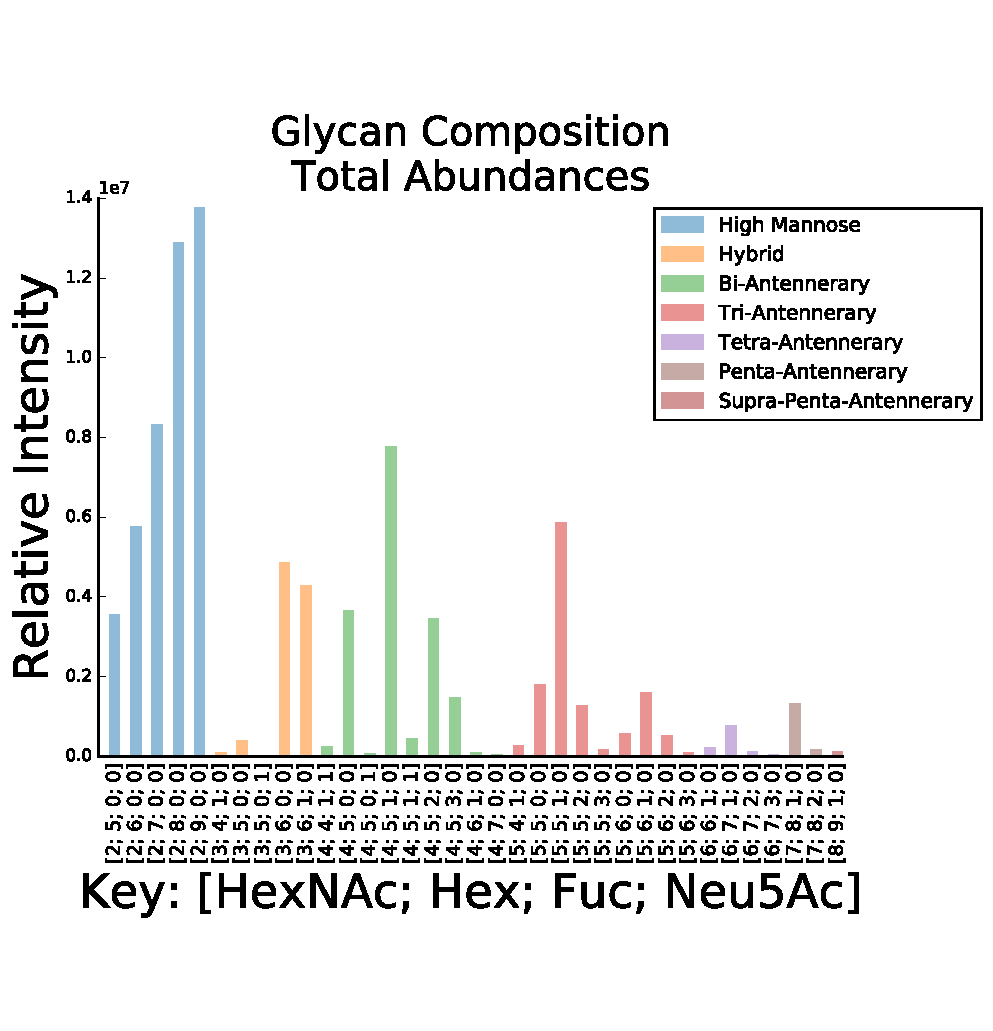
\includegraphics[width=0.45\textwidth,valign=t]{figure/phil_bs_abundances.pdf}
    \end{figure}

\begin{figure}[h]
    \caption{Performance Comparison with and without Network Smoothing for \philbs
             \label{fig:philbs_perf}}
    \centering
    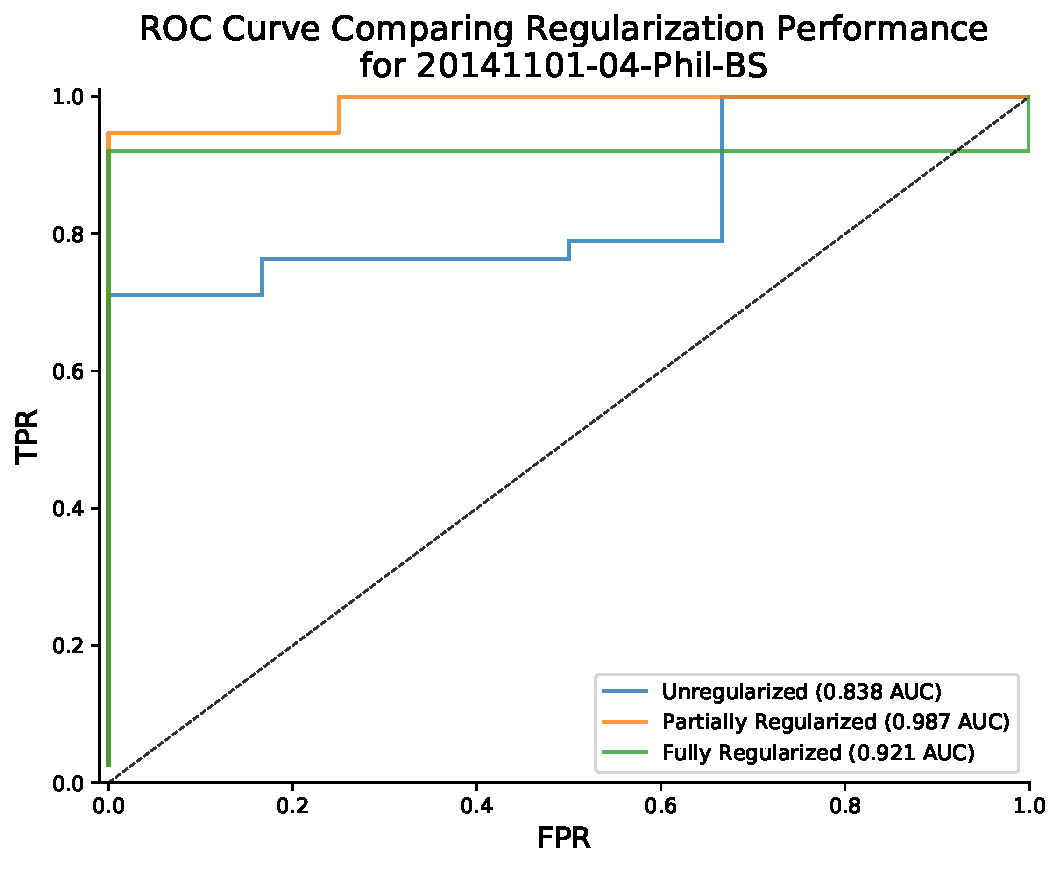
\includegraphics[width=0.42\textwidth,valign=t]{figure/phil_bs_native_roc.pdf}
    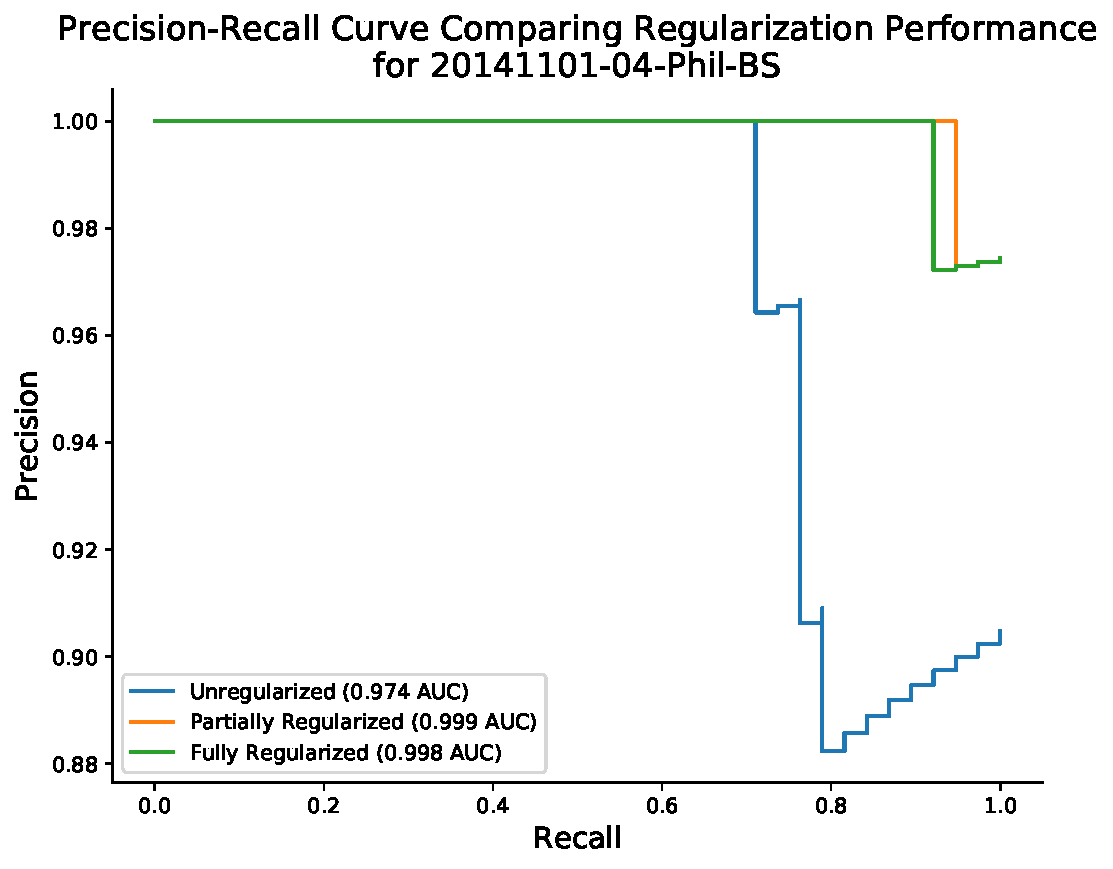
\includegraphics[width=0.45\textwidth,valign=t]{figure/phil_bs_native_prec_rec.pdf}
\end{figure}
